% ==============================================================================
% หน้าปกหนังสือวิชาการ ออกแบบเสมือนหน้าจอแอปพลิเคชันสมาร์ทโฟนระดับเรือธง (Flagship Smartphone UI)
% ชื่อหนังสือขนาดใหญ่พิเศษ 2.5 เท่า คมชัด โดดเด่น ทรงพลังระดับ Masterclass
% 100% สอดคล้องกับระเบียบวิชาการ ปลอดเครื่องหมายโคลอน (Zero Colon) ในภาษาไทย
% ==============================================================================
\thispagestyle{empty}
\begin{tikzpicture}[remember picture, overlay]

    % --------------------------------------------------------------------------
    % 1. ตัวเครื่องสมาร์ทโฟนและขอบเครื่องด้านนอก (Smartphone Titanium Chassis & Screen Bezel)
    % --------------------------------------------------------------------------
    % พื้นหลังขอบนอกสุด (ขอบเครื่องไทเทเนียมสี Dark Obsidian)
    \fill[color=black!96!rbruNavy] 
        (current page.south west) rectangle (current page.north east);

    % เส้นขอบแสงสะท้อนขอบโลหะรอบตัวเครื่อง
    \draw[color=green!60!rbruGold, line width=1.4pt, opacity=0.60, rounded corners=1.4cm] 
        ($(current page.south west) + (0.5cm, 0.5cm)$) rectangle ($(current page.north east) + (-0.5cm, -0.5cm)$);

    % หน้าจอดิจิทัลแบบ OLED ขอบมน (OLED Display Surface)
    \fill[top color=rbruNavy!98!black, bottom color=black, rounded corners=1.2cm] 
        ($(current page.south west) + (0.7cm, 0.7cm)$) rectangle ($(current page.north east) + (-0.7cm, -0.7cm)$);

    % รัศมีแสงเรืองรองนุ่มนวลด้านหลังอินเทอร์เฟซ (Soft Ambient Glow Behind UI)
    \fill[green!25, opacity=0.15] ($(current page.center) + (0, 3.2cm)$) circle (7.0cm);
    \fill[cyan!20, opacity=0.08] ($(current page.center) + (2.5cm, -3.2cm)$) circle (4.5cm);

    % --------------------------------------------------------------------------
    % 2. แถบสถานะสมาร์ทโฟน (Status Bar: Time, 5G, Dynamic Island, Battery)
    % --------------------------------------------------------------------------
    % เวลาและเครือข่ายฝั่งซ้าย
    \node[anchor=north west, align=left] at ($(current page.north west) + (1.6cm, -1.15cm)$) {
        {\fontsize{11}{13}\selectfont\bfseries\color{white} 09:41}\quad
        {\fontsize{9}{11}\selectfont\bfseries\color{green!80!white} 5G RBRU-AGRI}
    };

    % ไดนามิกไอแลนด์ตรงกลาง (Dynamic Island Pill Cutout)
    \node[anchor=north, align=center] at ($(current page.north) + (0, -1.0cm)$) {
        \begin{tikzpicture}
            % กรอบแคปซูลสีดำสนิทพร้อมเส้นขอบนีออนเรืองแสง
            \fill[black, rounded corners=3.8mm] (-2.3, -0.38) rectangle (2.3, 0.38);
            \draw[color=green!65!white, line width=0.8pt, rounded corners=3.8mm, opacity=0.8] (-2.3, -0.38) rectangle (2.3, 0.38);
            
            % เลนส์กล้องหน้าและเซนเซอร์
            \fill[blue!40!black] (-1.7, 0) circle (0.16cm);
            \fill[green!90!white] (-1.7, 0) circle (0.05cm);
            \fill[black!80] (-1.2, 0) circle (0.09cm);

            % ข้อความแสดงสถานะทำงาน AI ในแคปซูล
            \node[anchor=center] at (0.35, 0) {
                {\fontsize{8.5}{10}\selectfont\bfseries\color{green!85!white} $\bullet$\,\color{white} SOILPH-HT LIVE ATC}
            };
        \end{tikzpicture}
    };

    % สถานะแบตเตอรี่ Wi-Fi และ GPS ฝั่งขวา
    \node[anchor=north east, align=right] at ($(current page.north east) + (-1.6cm, -1.15cm)$) {
        {\fontsize{9}{11}\selectfont\color{white!90} BLE $\cdot$ Wi-Fi 6}\quad
        {\fontsize{10}{12}\selectfont\bfseries\color{green!85!white} [\,100\%\,\begin{tikzpicture}[baseline=-0.5ex, scale=0.65]\fill[color=yellow!90!orange] (0,0.2) -- (-0.08,0.02) -- (0.02,0.02) -- (-0.05,-0.2) -- (0.09,-0.01) -- (-0.01,-0.01) -- cycle;\end{tikzpicture}\,]}
    };

    % --------------------------------------------------------------------------
    % 3. แถบหัวแอปพลิเคชัน (App Top Bar: Series Badge)
    % --------------------------------------------------------------------------
    \node[anchor=north, align=center] at ($(current page.north) + (0, -2.15cm)$) {
        \begin{tikzpicture}
            % ป้ายชื่อชุดตำราวิชาการ RBRU Monograph
            \node[fill=rbruGold!20, draw=rbruGold!85, line width=0.9pt, rounded corners=3mm, text=rbruGold, inner sep=4pt] (badge) {
                {\fontsize{9}{12}\selectfont\bfseries RBRU DIGITAL AGRIPHYSICS MONOGRAPH SERIES (VOL. 3)}
            };
        \end{tikzpicture}
    };

    % --------------------------------------------------------------------------
    % 4. ส่วนแสดงชื่อหนังสือวิชาการหลัก (Main Title: ขนาดใหญ่ขึ้น 2.5 เท่า เด่นชัดสูงสุด)
    % --------------------------------------------------------------------------
    \node[anchor=north, align=center] at ($(current page.north) + (0, -2.95cm)$) {
        {\fontsize{14}{18}\selectfont\bfseries\color{rbruGold} ฟิสิกส์เกษตรดิจิทัลและการเรียนรู้เชิงลึก}\\[8pt]
        {\fontsize{42}{48}\selectfont\bfseries\color{white} คู่มือการพัฒนาแอปพลิเคชัน}\\[6pt]
        {\fontsize{42}{48}\selectfont\bfseries\color{cyan!90!white} SoilpH-HT AI}\\[6pt]
        {\fontsize{34}{40}\selectfont\bfseries\color{white} ตรวจวัดกรด-ด่างของดิน}\\[6pt]
        {\fontsize{30}{36}\selectfont\bfseries\color{green!85!white} ชดเชยอุณหภูมิและความชื้นด้วยโครงข่าย PINN}\\[10pt]
        {\color{rbruGold}\rule{0.68\textwidth}{1.5pt}}\\[7pt]
        {\fontsize{10.5}{14}\selectfont\color{white!85} SoilpH-HT: Smartphone Real-Time Soil pH Analysis with Live Stream,}\\[2pt]
        {\fontsize{10.5}{14}\selectfont\color{white!85} Temperature-Moisture Error Compensation via Deep PINN}
    };

    % --------------------------------------------------------------------------
    % 5. ช่องมองภาพกล้องสดและเรดาร์วิทัศน์ (Live Camera Viewfinder HUD Canvas)
    % บรรจุภาพถ่ายจริง jc_soil_ai_pr_vertical_9x16.jpg แปลงทุเรียนและเซนเซอร์จริง
    % --------------------------------------------------------------------------
    \node[anchor=center] at ($(current page.center) + (0, -1.8cm)$) {
        \begin{tikzpicture}
            % กรอบช่องมองภาพกล้อง (Camera Viewport Frame)
            \fill[black!65!rbruNavy, rounded corners=5.5mm] (-5.8, -2.25) rectangle (5.8, 2.25);
            \draw[green!65!white, line width=1.1pt, rounded corners=5.5mm, opacity=0.85] (-5.8, -2.25) rectangle (5.8, 2.25);

            % มุมกรอบช่วยเล็ง 4 มุม (HUD Camera Corner Brackets)
            \draw[color=green!90!white, line width=2.2pt] (-5.5, 1.75) -- (-5.5, 2.05) -- (-5.1, 2.05);
            \draw[color=green!90!white, line width=2.2pt] (5.5, 1.75) -- (5.5, 2.05) -- (5.1, 2.05);
            \draw[color=green!90!white, line width=2.2pt] (-5.5, -1.75) -- (-5.5, -2.05) -- (-5.1, -2.05);
            \draw[color=green!90!white, line width=2.2pt] (5.5, -1.75) -- (5.5, -2.05) -- (5.1, -2.05);

            % บรรจุภาพถ่ายจริงระบบตรวจวัดดินและหัววัดเซนเซอร์ในแปลงทุเรียน
            \begin{scope}
                \clip[rounded corners=4.5mm] (-5.65, -2.1) rectangle (5.65, 2.1);
                \node at (0, 0) {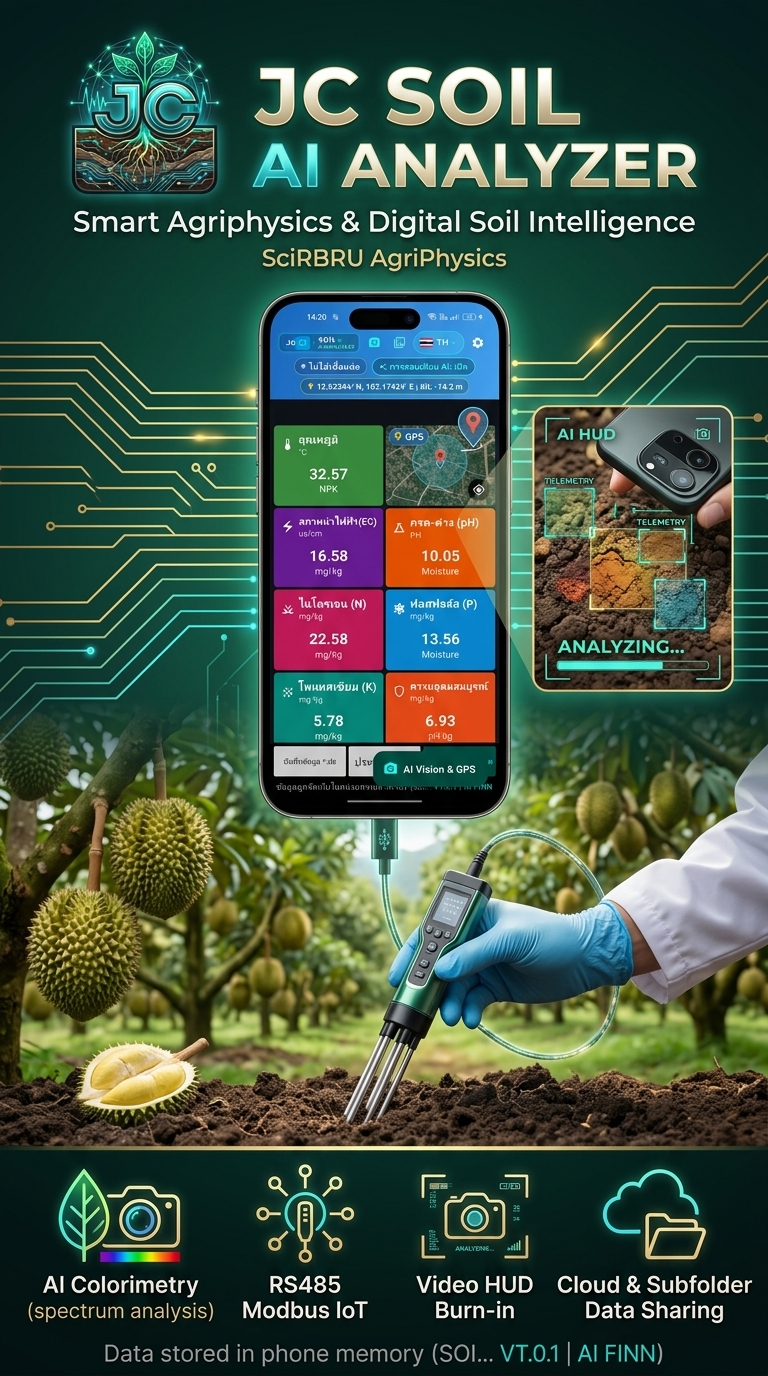
\includegraphics[width=11.4cm, height=4.3cm]{figures/jc_soil_ai_pr_vertical_9x16.jpg}};
                % เส้นแสงไล่ระดับเสริมความคมชัด
                \fill[left color=rbruNavy!35, right color=transparent, opacity=0.35] (-5.7, -2.2) rectangle (5.7, 2.2);
            \end{scope}

            % ข้อมูลโอเวอร์เลย์บนกล้อง (Telemetry HUD Overlays)
            \node[anchor=north west, fill=black!75, rounded corners=2mm, inner sep=2.5pt] at (-5.3, 1.95) {
                {\fontsize{7.5}{9}\selectfont\color{green!90!white} $\bullet$\,LIVE STREAM}\quad
                {\fontsize{7.5}{9}\selectfont\color{white} 60 FPS}\quad
                {\fontsize{7.5}{9}\selectfont\color{cyan!90!white} ROI หลายเหลี่ยม}
            };
            \node[anchor=north east, fill=black!75, rounded corners=2mm, inner sep=2.5pt] at (5.3, 1.95) {
                {\fontsize{7.5}{9}\selectfont\color{rbruGold} ชดเชยอุณหภูมิ Nernst ATC}
            };
            \node[anchor=south west, fill=black!75, rounded corners=2mm, inner sep=2.5pt] at (-5.3, -1.95) {
                {\fontsize{7.5}{9}\selectfont\color{cyan!90!white} แปลงทุเรียนเมืองจันท์}
            };
            \node[anchor=south east, fill=black!75, rounded corners=2mm, inner sep=2.5pt] at (5.3, -1.95) {
                {\fontsize{7.5}{9}\selectfont\color{green!90!white} ความแม่นยำ $R^2 \ge 0.96$}
            };
        \end{tikzpicture}
    };

    % --------------------------------------------------------------------------
    % 6. วิดเจ็ตแดชบอร์ดผลการวิเคราะห์ AI (Multimodal AI Telemetry Dashboard Card)
    % --------------------------------------------------------------------------
    \node[anchor=center] at ($(current page.center) + (0, -5.25cm)$) {
        \begin{tikzpicture}
            % กรอบ Glassmorphism Card
            \fill[rbruNavy!88!black, rounded corners=4.5mm] (-5.8, -1.25) rectangle (5.8, 1.25);
            \draw[white!25, line width=0.9pt, rounded corners=4.5mm] (-5.8, -1.25) rectangle (5.8, 1.25);

            % การ์ดย่อยที่ 1: ค่า pH เชิงแสง (Vision Optical pH)
            \node[fill=black!45, draw=cyan!60, rounded corners=3mm, inner sep=3.5pt, minimum width=2.65cm, minimum height=1.15cm] (c1) at (-4.2, 0.35) {
                \begin{tabular}{c}
                    {\fontsize{7}{8.5}\selectfont\color{cyan!90!white} pH เชิงแสง (Vision)}\\
                    {\fontsize{11.5}{13.5}\selectfont\bfseries\color{white} pH 6.48}\\
                    {\fontsize{6.5}{7.5}\selectfont\color{green!85!white} กรดเล็กน้อย}
                \end{tabular}
            };

            % การ์ดย่อยที่ 2: ค่า pH จากหัววัดเซนเซอร์จริง (Sensor Calibrated pH)
            \node[fill=black!45, draw=rbruGold!70, rounded corners=3mm, inner sep=3.5pt, minimum width=2.65cm, minimum height=1.15cm] (c2) at (-1.4, 0.35) {
                \begin{tabular}{c}
                    {\fontsize{7}{8.5}\selectfont\color{rbruGold} pH เซนเซอร์จริง}\\
                    {\fontsize{11.5}{13.5}\selectfont\bfseries\color{white} pH 6.60}\\
                    {\fontsize{6.5}{7.5}\selectfont\color{green!85!white} ชดเชย PINN แล้ว}
                \end{tabular}
            };

            % การ์ดย่อยที่ 3: ความสอดคล้อง (Consistency Delta pH)
            \node[fill=black!45, draw=green!70, rounded corners=3mm, inner sep=3.5pt, minimum width=2.65cm, minimum height=1.15cm] (c3) at (1.4, 0.35) {
                \begin{tabular}{c}
                    {\fontsize{7}{8.5}\selectfont\color{green!85!white} ตรวจสอบความสอดคล้อง}\\
                    {\fontsize{11.5}{13.5}\selectfont\bfseries\color{white} $\Delta\text{pH } 0.12$}\\
                    {\fontsize{6.5}{7.5}\selectfont\color{cyan!90!white} สอดคล้อง 98.2\%}
                \end{tabular}
            };

            % การ์ดย่อยที่ 4: ความชื้นและอุณหภูมิ (Humidity & Temp HT)
            \node[fill=black!45, draw=orange!70, rounded corners=3mm, inner sep=3.5pt, minimum width=2.65cm, minimum height=1.15cm] (c4) at (4.2, 0.35) {
                \begin{tabular}{c}
                    {\fontsize{7}{8.5}\selectfont\color{orange!85!white} อุณหภูมิและความชื้น}\\
                    {\fontsize{10.5}{12.5}\selectfont\bfseries\color{white} 28.5$^\circ\text{C}$ / 34.8\%}\\
                    {\fontsize{6.5}{7.5}\selectfont\color{orange!90!white} สภาวะแปลง เหมาะสม}
                \end{tabular}
            };

            % แถบล่างในวิดเจ็ต แสดงตัวแปรเซนเซอร์กายภาพ 7 มิติ
            \node[anchor=center] at (0, -0.72) {
                {\fontsize{7.2}{8.5}\selectfont\color{white!80} สถาปัตยกรรม PINN} \quad
                {\fontsize{7.2}{8.5}\selectfont\color{cyan!90!white} แรงดันไฟฟ้าเซนเซอร์ 24.8 mV} \quad
                {\fontsize{7.2}{8.5}\selectfont\color{white!40} $\cdot$} \quad
                {\fontsize{7.2}{8.5}\selectfont\color{cyan!90!white} ดัชนีความอุดมสมบูรณ์ 88.5\%} \quad
                {\fontsize{7.2}{8.5}\selectfont\color{white!40} $\cdot$} \quad
                {\fontsize{7.2}{8.5}\selectfont\color{green!90!white} บันทึกเรียบร้อย}
            };
        \end{tikzpicture}
    };

    % --------------------------------------------------------------------------
    % 7. แถบปุ่มควบคุมการทำงาน (Mobile App Bottom Navigation Bar)
    % --------------------------------------------------------------------------
    \node[anchor=center] at ($(current page.center) + (0, -7.0cm)$) {
        \begin{tikzpicture}
            % กรอบแถบนำทางด้านล่าง
            \fill[black!75, rounded corners=3.5mm] (-5.6, -0.38) rectangle (5.6, 0.38);
            \draw[white!20, line width=0.7pt, rounded corners=3.5mm] (-5.6, -0.38) rectangle (5.6, 0.38);

            % ปุ่มแท็บ 4 ปุ่ม
            \node at (-4.2, 0) {{\fontsize{7.8}{9.5}\selectfont\bfseries\color{cyan!90!white} [\,หน้าหลัก\,]}};
            \node at (-1.4, 0) {{\fontsize{7.8}{9.5}\selectfont\color{white!80} [\,หัววัดสด\,]}};
            \node at (1.4, 0) {{\fontsize{7.8}{9.5}\selectfont\color{white!80} [\,สอบเทียบ PINN\,]}};
            \node at (4.2, 0) {{\fontsize{7.8}{9.5}\selectfont\color{white!80} [\,คำแนะนำดิน\,]}};
        \end{tikzpicture}
    };

    % --------------------------------------------------------------------------
    % 8. ข้อมูลผู้เขียน สังกัด และแถบควบคุมโฮม (Author Metadata & Home Gesture Bar)
    % --------------------------------------------------------------------------
    \node[anchor=south, align=center] at ($(current page.south) + (0, 1.45cm)$) {
        {\fontsize{14}{18}\selectfont\bfseries\color{white} ผู้ช่วยศาสตราจารย์ ดร.ชีวะ ทัศนา}\\[2.5pt]
        {\fontsize{10.5}{13.5}\selectfont\color{rbruGold} สาขาวิชาฟิสิกส์ คณะวิทยาศาสตร์และเทคโนโลยี มหาวิทยาลัยราชภัฏรำไพพรรณี}\\[2pt]
        {\fontsize{8.5}{11}\selectfont\color{white!70} ศูนย์ความเป็นเลิศด้านฟิสิกส์เกษตรและเทคโนโลยีปัญญาประดิษฐ์ฝังตัว}
    };

    % แถบสัมผัสโฮมล่างสุดของสมาร์ทโฟน (Home Gesture Indicator Bar)
    \draw[color=white!60, line width=3.0pt, line cap=round] 
        ($(current page.south) + (-2.2cm, 0.95cm)$) -- ($(current page.south) + (2.2cm, 0.95cm)$);

\end{tikzpicture}
\clearpage
